\documentclass[a4paper]{article} 
\addtolength{\hoffset}{-2.25cm}
\addtolength{\textwidth}{4.5cm}
\addtolength{\voffset}{-3.25cm}
\addtolength{\textheight}{5cm}
\setlength{\parskip}{0pt}
\setlength{\parindent}{0in}

\usepackage{natbib}
\usepackage{blindtext} % Package to generate dummy text
\usepackage{charter} % Use the Charter font
\usepackage[utf8]{inputenc} % Use UTF-8 encoding
\usepackage{microtype} % Slightly tweak font spacing for aesthetics
\usepackage{amsthm, amsmath, amssymb} % Mathematical typesetting
\usepackage{float} % Improved interface for floating objects
\usepackage{hyperref} % For hyperlinks in the PDF
\usepackage{graphicx, multicol} % Enhanced support for graphics
\usepackage{xcolor} % Driver-independent color extensions
\usepackage{pseudocode} % Environment for specifying algorithms in a natural way
\usepackage[ddmmyyyy]{datetime} % Uses YEAR-MONTH-DAY format for dates
%\usepackage{gensymb}
\usepackage{bibentry}

\usepackage{fancyhdr} % Headers and footers
\pagestyle{fancy} % All pages have headers and footers
\fancyhead{}\renewcommand{\headrulewidth}{0pt} % Blank out the default header
\fancyfoot[L]{} % Custom footer text
\fancyfoot[C]{} % Custom footer text
\fancyfoot[R]{\thepage} % Custom footer text
\newcommand{\note}[1]{\marginpar{\scriptsize \textcolor{red}{#1}}} % Enables comments in red on margin

%----------------------------------------------------------------------------------------

\usepackage{adjustbox}
\usepackage{float}
\usepackage{multicol}
\usepackage{pgfplots, pgfplotstable}
%-------------------------------
%	TITLE VARIABLES (identify your work!)
%-------------------------------

\newcommand{\yourname}{Jakob Kralj 4.A} % replace YOURNAME with your name
\newcommand{\papertitle}{Sila Podlage} % replace X with paper title

\begin{document}

%-------------------------------
%	TITLE SECTION (do not modify unless you really need to)
%-------------------------------
\fancyhead[C]{}
\hrule \medskip
\begin{minipage}{0.295\textwidth} 
\raggedright
\footnotesize
\yourname \hfill\\ 
\end{minipage}
\begin{minipage}{0.69\textwidth} 
\centering 
\Large
\text{\papertitle}\\ 
\normalsize 
\end{minipage}
\medskip\hrule 
\bigskip


%-------------------------------
%	ASSIGNMENT CONTENT (add your responses)
%-------------------------------

\section*{Naloga:} % this is an example
Izmeri koeficient trenja ter koeficient lepenja.

\section*{Potrebščine:}

Klada z utežmi, silomer, podlaga z različnimi prevlekami.

\section*{Skica:}

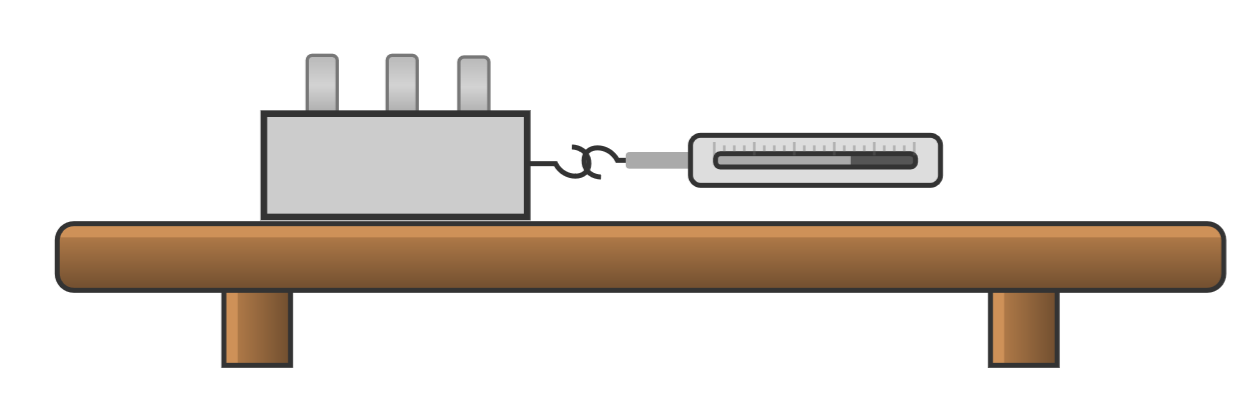
\includegraphics[scale=0.5]{skica.png}

\section*{Meritve:}

Klado, ki si ji izmeril maso, vleci s silo, ki je vzporedna s tlemi. Odčitaj vrednost sile v trenutku, ko se klada premakne. Ta sila je nasprotno enaka sili lepenja. Nato vleci klado s silo, ki je vzporedna s tlemi tako, da bo drsela enakomerno. Sila, ki jo  odčitaš na silomeru, je nasprotno enaka sili trenja. Meritve vnašaj v tabelo. Meritev izvedi za dve različni podlagi, za štiri različne teže klade (na klado polagaš uteži).

\begin{multicols}{2}

Podlaga 1
\begin{table}[H]
\centering
\renewcommand{\arraystretch}{1.5}
\begin{tabular}{lll}
   m(klade)$[g]$ & $F_{lepenja}[N]$ & $F_{trenja}[N]$ \\
   435  & 2 & 1 \\
   925  & 4 & 2 \\
   1415 & 6 & 3 \\
   1905 & 8 & 4
\end{tabular}
\end{table}

\columnbreak

Podlaga 2
\begin{table}[H]
\centering
\renewcommand{\arraystretch}{1.5}
\begin{tabular}{lll}
   m(klade)$[g]$ & $F_{lepenja}[N]$ & $F_{trenja}[N]$ \\
435  & 3  & 2 \\
925  & 6  & 5   \\
1415 & 9  & 7   \\
1905 & 13 & 10 
\end{tabular}
\end{table}

\end{multicols}
\section*{Rezultati in obdelava podatkov:}

\begin{multicols}{2}
$k$ lahko izračunamo s pomočjo formule:
\begin{equation}
   k = \frac{F}{mg}
\end{equation}

\columnbreak

Kjer lahko uporabimo parametre:
\begin{gather}
   g = 9.81ms^-2
\end{gather}

\end{multicols}

Iz tega sledijo rezultati:

Podlaga 1

\begin{multicols}{2}
   \begin{table}[H]
      \begin{tabular}{lllll}
         $m(klade)[kg]$ & $F_{lepenja}[N]$ & $F_{trenja}[N]$ & $k_{lepenja}$ & $k_{trenja}$\\
         0,435 & 2 & 1 & 0,70 & 0,23 \\
         0,925 & 4 & 2 & 0,44 & 0,22 \\
         1,415 & 6 & 3 & 0,43 & 0,22 \\
         1,905 & 8 & 4 & 0,43 & 0,21
      \end{tabular}
      \end{table}
   \columnbreak
   \begin{gather}
      k_{trenja} = 0,22 \pm 0,01 \\
      k_{trenja} = 0,22 (1 \pm 0.05) \\
      k_{lepenja} = 0,44 \pm 0.03 \\
      k_{lepenja} = 0,44(1 \pm 0.7) \\
   \end{gather}
   \columnbreak
\end{multicols}
\begin{multicols}{2}
\pgfplotstableread{
X Y
4.2 2
9.0 4
13.9 6
18.7 8
}\datatable

\begin{center}
\begin{tikzpicture}
\begin{axis}[
   legend pos= north west,
   title = {$F_{l}(F_n)$},
   xlabel={$F_{n}[N]$},
   ylabel={$F_{l}[N]$}
   ]
\addplot [only marks, mark = *] table {\datatable};
\addplot [thick, red] table[
    y={create col/linear regression={y=Y}}
] % compute a linear regression from the input table
{\datatable};
\addlegendentry{$m(V)$}
\addlegendentry{%
$\pgfmathprintnumber{\pgfplotstableregressiona} \cdot x
\pgfmathprintnumber[print sign]{\pgfplotstableregressionb}$}
\end{axis}
\end{tikzpicture}
\end{center}
\columnbreak
\pgfplotstableread{
X Y
4.2 1
9.0 2
13.9 3
18.7 4
}\datatable

\begin{center}
\begin{tikzpicture}
\begin{axis}[
   legend pos= north west,
   title = {$F_{tr}(F_n)$},
   xlabel={$F_{n}[N]$},
   ylabel={$F_{tr}[N]$}
   ]
\addplot [only marks, mark = *] table {\datatable};
\addplot [thick, red] table[
    y={create col/linear regression={y=Y}}
] % compute a linear regression from the input table
{\datatable};
\addlegendentry{$m(V)$}
\addlegendentry{%
$\pgfmathprintnumber{\pgfplotstableregressiona} \cdot x
\pgfmathprintnumber[print sign]{\pgfplotstableregressionb}$}
\end{axis}
\end{tikzpicture}
\end{center}
\end{multicols}
Podlaga 2

\begin{multicols}{2}
   \begin{table}[H]
      \begin{tabular}{lllll}
         $m(klade)[kg]$ & $F_{lepenja}[N]$ & $F_{trenja}[N]$ & $k_{lepenja}$ & $k_{trenja}$\\
         0,435 & 3  & 2 & 0,70 & 0,52 \\
         0,925 & 6  & 5   & 0,66 & 0,55 \\
         1,415 & 9  & 7   & 0,65 & 0,50 \\
         1,905 & 13 & 10  & 0,70 & 0,54
      \end{tabular}
      \end{table}
   \columnbreak
   \begin{gather}
      k_{trenja} = 0,53 \pm 0,05 \\
      k_{trenja} = 0,53(1 \pm 0.01) \\
      k_{lepenja} = 0,68 \pm 0.03 \\
      k_{lepenja} = 0,68(1 \pm 0.04) \\
   \end{gather}
   \columnbreak
\end{multicols}

\begin{multicols}{2}
\pgfplotstableread{
X Y
4.2 3
9.0 6
13.9 9
18.7 13
}\datatable

\begin{center}
\begin{tikzpicture}
\begin{axis}[
   legend pos= north west,
   title = {$F_{l}(F_n)$},
   xlabel={$F_{n}[N]$},
   ylabel={$F_{l}[N]$}
   ]
\addplot [only marks, mark = *] table {\datatable};
\addplot [thick, red] table[
      y={create col/linear regression={y=Y}}
] % compute a linear regression from the input table
{\datatable};
\addlegendentry{$m(V)$}
\addlegendentry{%
$\pgfmathprintnumber{\pgfplotstableregressiona} \cdot x
\pgfmathprintnumber[print sign]{\pgfplotstableregressionb}$}
\end{axis}
\end{tikzpicture}
\end{center}
\columnbreak
\pgfplotstableread{
X Y
4.2 2.2
9.0 5
13.9 7
18.7 10
}\datatable

\begin{center}
\begin{tikzpicture}
\begin{axis}[
   legend pos= north west,
   title = {$F_{tr}(F_n)$},
   xlabel={$F_{n}[N]$},
   ylabel={$F_{tr}[N]$}
   ]
\addplot [only marks, mark = *] table {\datatable};
\addplot [thick, red] table[
      y={create col/linear regression={y=Y}}
] % compute a linear regression from the input table
{\datatable};
\addlegendentry{$m(V)$}
\addlegendentry{%
$\pgfmathprintnumber{\pgfplotstableregressiona} \cdot x
\pgfmathprintnumber[print sign]{\pgfplotstableregressionb}$}
\end{axis}
\end{tikzpicture}
\end{center}
\end{multicols}



\section*{Interpretacija:}

Napaka je glede na pogoje eksperimenta sprejemljiva. Eden izmed glavnih razlogov za njen obstoj je nenatančnost merjenja s silo mera, branja direktno ob zdrsu in neenakomernost vleke v času merjenja trenja.

\end{document}